


\tikzset{every picture/.style={line width=0.75pt}} %set default line width to 0.75pt        

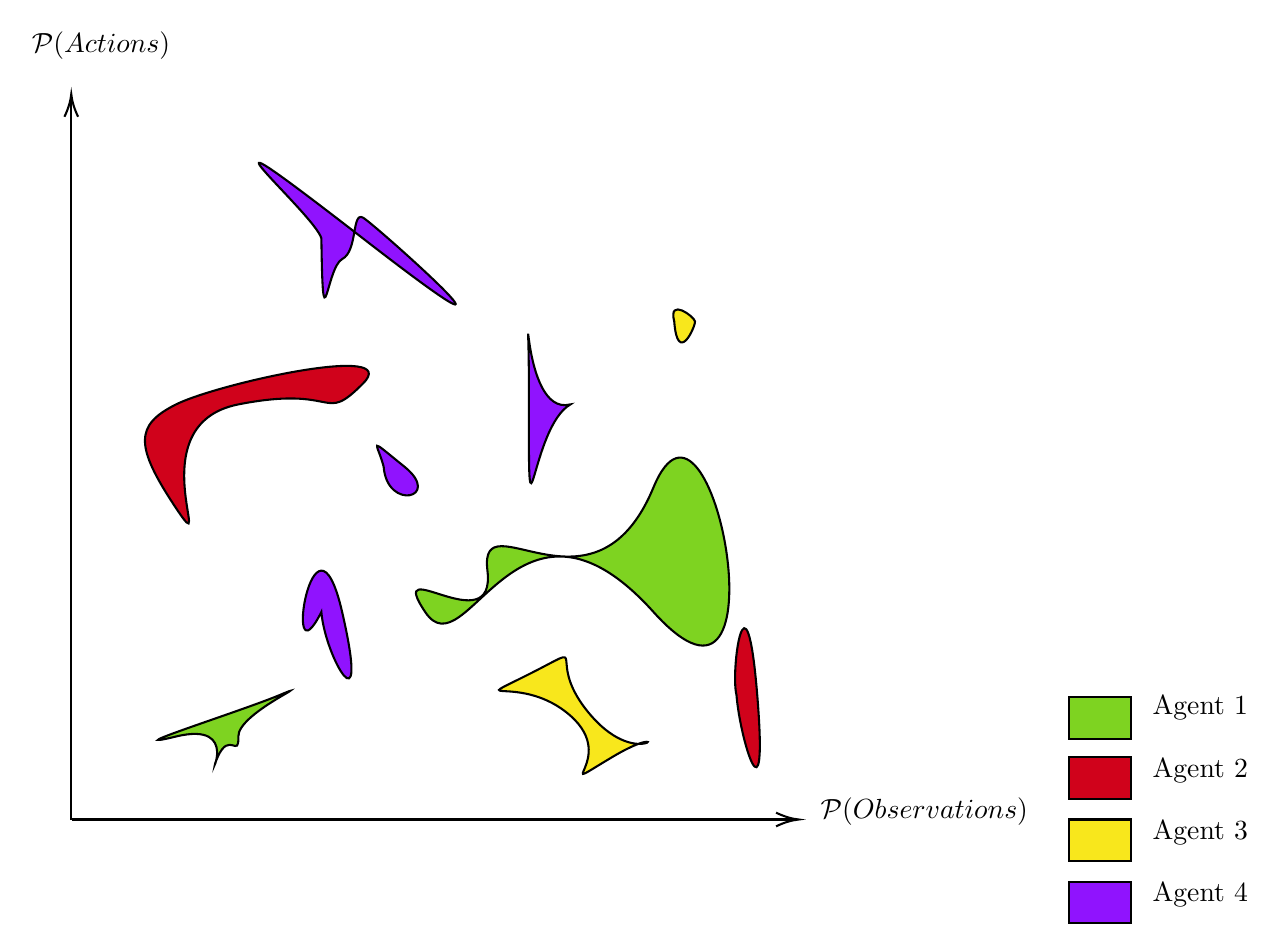
\begin{tikzpicture}[x=0.75pt,y=0.75pt,yscale=-1,xscale=1]
%uncomment if require: \path (0,488); %set diagram left start at 0, and has height of 488

%Straight Lines [id:da04410225677310331] 
\draw    (200,400) -- (548,400) ;
\draw [shift={(550,400)}, rotate = 180] [color={rgb, 255:red, 0; green, 0; blue, 0 }  ][line width=0.75]    (10.93,-3.29) .. controls (6.95,-1.4) and (3.31,-0.3) .. (0,0) .. controls (3.31,0.3) and (6.95,1.4) .. (10.93,3.29)   ;
%Shape: Boxed Line [id:dp05306980327962996] 
\draw    (199.5,400) -- (199.5,52.5) ;
\draw [shift={(199.5,50.5)}, rotate = 90] [color={rgb, 255:red, 0; green, 0; blue, 0 }  ][line width=0.75]    (10.93,-3.29) .. controls (6.95,-1.4) and (3.31,-0.3) .. (0,0) .. controls (3.31,0.3) and (6.95,1.4) .. (10.93,3.29)   ;
%Shape: Polygon Curved [id:ds08747541265856107] 
\draw  [fill={rgb, 255:red, 208; green, 2; blue, 27 }  ,fill opacity=1 ] (250,200) .. controls (270,190) and (360,170) .. (340,190) .. controls (320,210) and (329,190.33) .. (280,200) .. controls (231,209.67) and (270,280) .. (250,250) .. controls (230,220) and (230,210) .. (250,200) -- cycle ;
%Shape: Polygon Curved [id:ds4597838047306486] 
\draw  [fill={rgb, 255:red, 126; green, 211; blue, 33 }  ,fill opacity=1 ] (400,280) .. controls (395.67,244.33) and (451.67,308.33) .. (480,240) .. controls (508.33,171.67) and (545.67,373) .. (480,300) .. controls (414.33,227) and (390,330) .. (370,300) .. controls (350,270) and (404.33,315.67) .. (400,280) -- cycle ;
%Shape: Polygon Curved [id:ds8099729429831757] 
\draw  [fill={rgb, 255:red, 126; green, 211; blue, 33 }  ,fill opacity=1 ] (300,340) .. controls (318.33,332.33) and (279.67,349) .. (280,360) .. controls (280.33,371) and (275.67,357) .. (270,370) .. controls (264.33,383) and (281.67,352.33) .. (250,360) .. controls (218.33,367.67) and (281.67,347.67) .. (300,340) -- cycle ;
%Curve Lines [id:da8764285872929987] 
\draw [fill={rgb, 255:red, 248; green, 231; blue, 28 }  ,fill opacity=1 ]   (490,160) .. controls (487,148.33) and (499.67,157.67) .. (500,160) .. controls (500.33,162.33) and (491.67,181.67) .. (490,160) -- cycle ;
%Shape: Polygon Curved [id:ds4837178284217645] 
\draw  [fill={rgb, 255:red, 248; green, 231; blue, 28 }  ,fill opacity=1 ] (420,330) .. controls (452.2,313.8) and (425.8,322.2) .. (450,350) .. controls (474.2,377.8) and (491.8,351) .. (460,370) .. controls (428.2,389) and (463.8,371) .. (440,350) .. controls (416.2,329) and (387.8,346.2) .. (420,330) -- cycle ;
%Curve Lines [id:da4454812773064518] 
\draw [fill={rgb, 255:red, 144; green, 19; blue, 254 }  ,fill opacity=1 ]   (440,200) .. controls (414.6,206.6) and (420.2,120.2) .. (420,200) .. controls (419.8,279.8) and (420.6,211) .. (440,200) -- cycle ;
%Curve Lines [id:da941827926410739] 
\draw [fill={rgb, 255:red, 144; green, 19; blue, 254 }  ,fill opacity=1 ]   (320,300) .. controls (301,337.8) and (316.2,240.2) .. (330,300) .. controls (343.8,359.8) and (321.67,321.67) .. (320,300) -- cycle ;
%Curve Lines [id:da5126937457791156] 
\draw [fill={rgb, 255:red, 144; green, 19; blue, 254 }  ,fill opacity=1 ]   (350,230) .. controls (347,218.33) and (341.4,215) .. (360,230) .. controls (378.6,245) and (351.67,251.67) .. (350,230) -- cycle ;
%Curve Lines [id:da16147821661528838] 
\draw [fill={rgb, 255:red, 144; green, 19; blue, 254 }  ,fill opacity=1 ]   (320,120) .. controls (317,108.33) and (242.2,44.2) .. (340,120) .. controls (437.8,195.8) and (345.47,112.9) .. (340,110) .. controls (334.53,107.1) and (337.62,126.08) .. (330,130) .. controls (322.38,133.92) and (320.77,175.22) .. (320,120) -- cycle ;
%Curve Lines [id:da5113003951161588] 
\draw [fill={rgb, 255:red, 208; green, 2; blue, 27 }  ,fill opacity=1 ]   (520,340) .. controls (517,328.33) and (524.6,273.8) .. (530,340) .. controls (535.4,406.2) and (521.67,361.67) .. (520,340) -- cycle ;
%Shape: Rectangle [id:dp2340961425768744] 
\draw  [fill={rgb, 255:red, 126; green, 211; blue, 33 }  ,fill opacity=1 ] (680,341) -- (710,341) -- (710,361) -- (680,361) -- cycle ;
%Shape: Rectangle [id:dp9520708107807885] 
\draw  [fill={rgb, 255:red, 248; green, 231; blue, 28 }  ,fill opacity=1 ] (680,400) -- (710,400) -- (710,420) -- (680,420) -- cycle ;
%Shape: Rectangle [id:dp16463762436683327] 
\draw  [fill={rgb, 255:red, 208; green, 2; blue, 27 }  ,fill opacity=1 ] (680,370) -- (710,370) -- (710,390) -- (680,390) -- cycle ;
%Shape: Rectangle [id:dp1461538508882101] 
\draw  [fill={rgb, 255:red, 144; green, 19; blue, 254 }  ,fill opacity=1 ] (680,430) -- (710,430) -- (710,450) -- (680,450) -- cycle ;

% Text Node
\draw (179,19) node [anchor=north west][inner sep=0.75pt]   [align=left] {$\mathcal{P}(Actions)$};
% Text Node
\draw (559,388) node [anchor=north west][inner sep=0.75pt]   [align=left] {$\mathcal{P}(Observations)$};
% Text Node
\draw (719,339) node [anchor=north west][inner sep=0.75pt]   [align=left] {Agent 1};
% Text Node
\draw (719,369) node [anchor=north west][inner sep=0.75pt]   [align=left] {Agent 2};
% Text Node
\draw (719,399) node [anchor=north west][inner sep=0.75pt]   [align=left] {Agent 3};
% Text Node
\draw (719,429) node [anchor=north west][inner sep=0.75pt]   [align=left] {Agent 4};


\end{tikzpicture}